% This file was created with tikzplotlib v0.10.1.
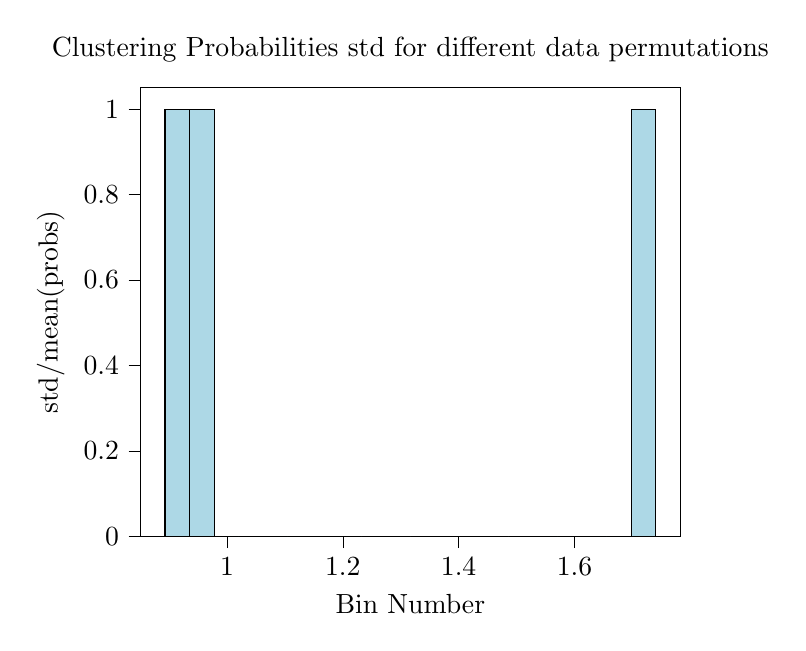
\begin{tikzpicture}

\definecolor{darkgray176}{RGB}{176,176,176}
\definecolor{lightblue}{RGB}{173,216,230}

\begin{axis}[
tick align=outside,
tick pos=left,
title={Clustering Probabilities std for different data permutations},
x grid style={darkgray176},
xlabel={Bin Number},
xmin=0.850739286864248, xmax=1.78244334883248,
xtick style={color=black},
y grid style={darkgray176},
ylabel={std/mean(probs)},
ymin=0, ymax=1.05,
ytick style={color=black}
]
\draw[draw=black,fill=lightblue] (axis cs:0.893089471499168,0) rectangle (axis cs:0.935439656134088,1);
\draw[draw=black,fill=lightblue] (axis cs:0.935439656134088,0) rectangle (axis cs:0.977789840769007,1);
\draw[draw=black,fill=lightblue] (axis cs:0.977789840769007,0) rectangle (axis cs:1.02014002540393,0);
\draw[draw=black,fill=lightblue] (axis cs:1.02014002540393,0) rectangle (axis cs:1.06249021003885,0);
\draw[draw=black,fill=lightblue] (axis cs:1.06249021003885,0) rectangle (axis cs:1.10484039467377,0);
\draw[draw=black,fill=lightblue] (axis cs:1.10484039467377,0) rectangle (axis cs:1.14719057930869,0);
\draw[draw=black,fill=lightblue] (axis cs:1.14719057930869,0) rectangle (axis cs:1.18954076394361,0);
\draw[draw=black,fill=lightblue] (axis cs:1.18954076394361,0) rectangle (axis cs:1.23189094857853,0);
\draw[draw=black,fill=lightblue] (axis cs:1.23189094857853,0) rectangle (axis cs:1.27424113321345,0);
\draw[draw=black,fill=lightblue] (axis cs:1.27424113321345,0) rectangle (axis cs:1.31659131784836,0);
\draw[draw=black,fill=lightblue] (axis cs:1.31659131784836,0) rectangle (axis cs:1.35894150248328,0);
\draw[draw=black,fill=lightblue] (axis cs:1.35894150248328,0) rectangle (axis cs:1.4012916871182,0);
\draw[draw=black,fill=lightblue] (axis cs:1.4012916871182,0) rectangle (axis cs:1.44364187175312,0);
\draw[draw=black,fill=lightblue] (axis cs:1.44364187175312,0) rectangle (axis cs:1.48599205638804,0);
\draw[draw=black,fill=lightblue] (axis cs:1.48599205638804,0) rectangle (axis cs:1.52834224102296,0);
\draw[draw=black,fill=lightblue] (axis cs:1.52834224102296,0) rectangle (axis cs:1.57069242565788,0);
\draw[draw=black,fill=lightblue] (axis cs:1.57069242565788,0) rectangle (axis cs:1.6130426102928,0);
\draw[draw=black,fill=lightblue] (axis cs:1.6130426102928,0) rectangle (axis cs:1.65539279492772,0);
\draw[draw=black,fill=lightblue] (axis cs:1.65539279492772,0) rectangle (axis cs:1.69774297956264,0);
\draw[draw=black,fill=lightblue] (axis cs:1.69774297956264,0) rectangle (axis cs:1.74009316419756,1);
\end{axis}

\end{tikzpicture}
